% Exact LaTeX recreation of the supplied Phase-1.pdf 
% Compile with pdfLaTeX. Place member pictures in the same folder if required.

\documentclass[11pt,a4paper]{article}

\usepackage[a4paper,left=2.0cm,right=2.0cm,top=1.55cm,bottom=1.55cm]{geometry}
\usepackage[T1]{fontenc}
\usepackage{lmodern}
\usepackage{graphicx}
\usepackage{xcolor}
\usepackage{array}
\usepackage{tabularx}
\usepackage{ragged2e}
\usepackage{enumitem}
\usepackage{fancyhdr}
\usepackage{tikz}
\usetikzlibrary{positioning, arrows.meta, shapes.geometric}
\usepackage{setspace}


% -------------------------------------------------
% COLOURS
% -------------------------------------------------
\definecolor{TitleBlue}{RGB}{61,103,154}

% -------------------------------------------------
% GENERAL SETTINGS
% -------------------------------------------------
\setlength{\parindent}{0pt}
\setlength{\parskip}{0pt}
\renewcommand{\arraystretch}{1.0}

% The supplied document uses a clean sans-serif heading style
% and italic serif-style explanatory text.
\newcommand{\blueheading}[1]{%
{\sffamily\color{TitleBlue}\fontsize{15}{18}\selectfont #1}%
}

\newcommand{\bluebigheading}[1]{%
{\sffamily\bfseries\color{TitleBlue}\fontsize{16}{19}\selectfont #1}%
}

% Auto-adjusting box for the text with tightened spacing
\newcommand{\answerbox}[2][]{%
\vspace{1pt}
\noindent
\fbox{%
\begin{minipage}[t]{\dimexpr\textwidth-2\fboxsep-2\fboxrule\relax}
\vspace{1mm}
\itshape #2
\vspace{1mm}
\end{minipage}
}
}

% -------------------------------------------------
% HEADER / FOOTER
% -------------------------------------------------
\pagestyle{fancy}
\fancyhf{}
\renewcommand{\headrulewidth}{0pt}
\renewcommand{\footrulewidth}{0pt}

\fancyhead[L]{%
\sffamily\bfseries\itshape\fontsize{10.5}{12}\selectfont
DSCPP-III-2026
}
\fancyhead[R]{%
\sffamily\bfseries\fontsize{10.5}{12}\selectfont
PROJECT PROPOSAL
}
\fancyfoot[R]{%
\itshape\fontsize{10}{12}\selectfont
Page \thepage
}
\setlength{\headheight}{14pt}
\setlength{\headsep}{23pt}
\setlength{\footskip}{24pt}

% -------------------------------------------------
% PAGE 1
% -------------------------------------------------
\begin{document}



\vspace*{4mm}

\bluebigheading{PROJECT AND TEAM INFORMATION}

\vspace{13mm}

\blueheading{Project Title}

\vspace{1mm}

\answerbox{Smart Driver Drowsiness \& Safety System}

\vspace{13mm}

\blueheading{Student / Team Information}

\vspace{2mm}

% -------------------------------------------------
% CORRECTED TABLE LAYOUT (Top-Aligned Text and Photos)
% -------------------------------------------------
\noindent
\begin{tabularx}{\textwidth}{|>{\RaggedRight\arraybackslash}p{0.75\textwidth}|>{\centering\arraybackslash}X|}
\hline
\begin{minipage}[t]{\linewidth}
\vspace{0pt}\vspace{1.5mm}
\textit{Team Name: \textbf{Smart Safety Team}}\\[0.5mm]
\textit{Team \#: \textbf{DSCPP-III-2026-T234}}
\vspace{1.5mm}
\end{minipage}
&
\begin{minipage}[t]{\linewidth}
\vspace{0pt}\vspace{1.5mm}
\textit{Photo}
\vspace{1.5mm}
\end{minipage}
\\
\hline
% ------------- TEAM MEMBER 1 -------------
\begin{minipage}[t]{\linewidth}
\vspace{0pt}\vspace{1.5mm}
\textbf{Team Member 1 (Team Lead)}\\[0.5mm]
\textit{Name: RIDVIK GARG}\\
\textit{University Roll No.: 2028039}\\
\textit{Section: H}\\
\textit{Email: ridvikridvik74@gmail.com}
\vspace{1.5mm}
\end{minipage}
&
\begin{minipage}[t]{\linewidth}
\vspace{0pt}\vspace{1.5mm}
\centering
\includegraphics[width=2.5cm,height=3.5cm,keepaspectratio]{member1.png}
\vspace{1.5mm}
\end{minipage}
\\
\hline
% ------------- TEAM MEMBER 2 -------------
\begin{minipage}[t]{\linewidth}
\vspace{0pt}\vspace{1.5mm}
\textbf{Team Member 2}\\[0.5mm]
\textit{Name: Prabhav Gulyani}\\
\textit{University Roll No.: 2027975}\\
\textit{Section: E}\\
\textit{Email: Prabhav7424@gmail.com}
\vspace{1.5mm}
\end{minipage}
&
\begin{minipage}[t]{\linewidth}
\vspace{0pt}\vspace{1.5mm}
\centering
\includegraphics[width=2.5cm,height=3.5cm,keepaspectratio]{member2.png}
\vspace{1.5mm}
\end{minipage}
\\
\hline
% ------------- TEAM MEMBER 3 -------------
\begin{minipage}[t]{\linewidth}
\vspace{0pt}\vspace{1.5mm}
\textbf{Team Member 3}\\[0.5mm]
\textit{Name: Nandini Gupta}\\
\textit{University Roll No.: 2028777}\\
\textit{Section: ML4}\\
\textit{Email: nandinigupta787@gmail.com}
\vspace{1.5mm}
\end{minipage}
&
\begin{minipage}[t]{\linewidth}
\vspace{0pt}\vspace{1.5mm}
\centering
\includegraphics[width=2.5cm,height=3.5cm,keepaspectratio]{member3.png}
\vspace{1.5mm}
\end{minipage}
\\
\hline
% ------------- TEAM MEMBER 4 -------------
\begin{minipage}[t]{\linewidth}
\vspace{0pt}\vspace{1.5mm}
\textbf{Team Member 4}\\[0.5mm]
\textit{Name: Antriksh Gehlot}\\
\textit{University Roll No.: 2028648}\\
\textit{Section: ML3}\\
\textit{Email: antrikshgehlot9290@gmail.com}
\vspace{1.5mm}
\end{minipage}
&
\begin{minipage}[t]{\linewidth}
\vspace{0pt}\vspace{1.5mm}
\centering
\includegraphics[width=2.5cm,height=3.5cm,keepaspectratio]{member4.png}
\vspace{1.5mm}
\end{minipage}
\\
\hline
\end{tabularx}

\vspace{5mm}
\noindent \textit{Mentor: Mr. Kamal Kumar Gola}

\newpage

% -------------------------------------------------
% PAGE 2
% -------------------------------------------------

\bluebigheading{PROPOSAL DESCRIPTION (10 pts)}

\vspace{4mm}

\blueheading{Motivation (1 pt)}

\vspace{1mm}

\answerbox{We selected driver safety as our project topic because a tired driver may lose attention on the road. This is more likely on long journeys, at night, or on roads where there is not much change. Our system will keep checking the driver and look for signs of sleepiness or distraction. It can give a warning, change the music when needed, save the event, and show the current safety condition. If the situation becomes serious, it can send a message to the saved family contact. This project also lets us use the topics we are learning, such as Data Structures, C++, Operating System concepts, and DBMS.}

\vspace{4mm}

\blueheading{State of the Art / Current solution (1 pt)}

\vspace{1mm}

\answerbox{Cars already have systems that use cameras or sensors to keep an eye on the driver. Some of them give a sound or screen warning when the driver looks tired. But many small projects focus on only one thing. for example checking closed eyes and giving an alarm.\newline Our prototype is planned to handle more than one task. It will check for drowsiness as well as distraction. Depending on the condition, it will give a warning, control the music, and save the event. It will also show whether the driver is in Good, Warning, or Critical condition. For storing and handling the information, we plan to use Queue, Stack, Linked List, and SQLite.}

\vspace{4mm}

\blueheading{Project Goals and Milestones (2 pts)}

\vspace{1mm}

\answerbox{Our main aim is to build a driver safety prototype that can detect possible drowsiness or distraction and respond to it.\newline Main goals: 1. Check if the driver's eyes stay closed for too long. 2. Check if the driver keeps looking away for too long. 3. Give a normal warning first and a stronger alert if needed. 4. Lower or pause the music during an unsafe condition. 5. Send a message to the saved family contact in a critical case. 6. Store drowsiness, distraction, and alert events. 7. Display the status as Good, Warning, or Critical. Milestones: 1. Understand the requirements and decide the modules. 2. Work on the drowsiness and distraction part. 3. Add alerts, music control, and the family message feature. 4. Use Queue, Stack, Linked List, and SQLite for the required data. 5. Connect the modules, test them, remove errors, and prepare the prototype.}

\vspace{4mm}

\blueheading{Project Approach (3 pts)}

\vspace{1mm}

\answerbox{We plan to make the project module by module. First, we will build each part and test it separately. Once the parts work, we will connect them.\newline The camera will capture the driver's face. From the face and eyes, the program will check for signs of sleepiness. It will also check if the driver is looking away for a longer time.\newline If the driver seems sleepy or distracted, the system will give a warning. If the same condition continues, the alert level will increase. In a serious case, a message can be sent to the family contact. The music can also be reduced or stopped so that the warning is easier to notice.\newline For data handling, a Linked List will keep the warning and event records. Queue and Stack will be used in places where they fit the task. We will make C++ classes for the different parts of the program. Threads will allow monitoring and alert work to run at the same time.\newline OpenCV will be used for the camera and face/eye detection. SQLite will keep driver information, contact information, and event records. We will code in C++ in VS Code and use GitHub for the project files.\newline At the end, we will connect everything and test the full system before preparing the prototype.}

\newpage

% -------------------------------------------------
% PAGE 3
% -------------------------------------------------

\blueheading{System Architecture (High Level Diagram)(2 pts)}

\vspace{2mm}

\begin{center}
\resizebox{0.75\linewidth}{!}{
\begin{tikzpicture}[
    node distance=0.8cm and 0.4cm,
    box/.style={draw, rounded corners, minimum width=2.8cm, minimum height=0.7cm, align=center, font=\normalfont\small},
    arrow/.style={->, >=stealth, thick}
]

% Nodes
\node[box] (camera) {Camera Input};
\node[box, below=0.6cm of camera] (monitor) {Driver Monitoring};
\node[box, below=1cm of monitor] (event) {Event Manager};
\node[box, left=1cm of event] (drowsy) {Drowsiness Detection};
\node[box, right=1cm of event] (distract) {Distraction Detection};

\node[box, below=1cm of event] (stack) {Stack\\Recent Alerts};
\node[box, left=0.5cm of stack] (queue) {Queue\\Safety Events};
\node[box, right=0.5cm of stack] (linked) {Linked List\\Event History};

\node[box, below=1cm of stack] (alert) {Alert Manager};

\node[box, below=1cm of alert] (music) {Automatic Music Control};
\node[box, left=0.5cm of music] (warning) {Warning / Alarm};
\node[box, right=0.5cm of music] (emergency) {Emergency Family Message};

\node[box, below=1cm of music, minimum width=12cm] (sqlite) {SQLite Database\\Driver + Contacts + Events + Safety Score};

% Arrows
\draw[arrow] (camera) -- (monitor);
\draw[arrow] (monitor) -- (drowsy);
\draw[arrow] (monitor) -- (distract);
\draw[arrow] (drowsy) -- (event);
\draw[arrow] (distract) -- (event);
\draw[arrow] (event) -- (queue);
\draw[arrow] (event) -- (stack);
\draw[arrow] (event) -- (linked);
\draw[arrow] (queue) -- (alert);
\draw[arrow] (stack) -- (alert);
\draw[arrow] (linked) -- (alert);
\draw[arrow] (alert) -- (warning);
\draw[arrow] (alert) -- (music);
\draw[arrow] (alert) -- (emergency);
\draw[arrow] (warning) |- (sqlite);
\draw[arrow] (music) -- (sqlite);
\draw[arrow] (emergency) |- (sqlite);

\end{tikzpicture}
}
\end{center}

\vspace{4mm}

\blueheading{Project Outcome / Deliverables (1 pts)}

\vspace{1mm}

\answerbox{We expect to have a working prototype of the Smart Driver Drowsiness Safety System. It should monitor the driver, identify possible drowsiness or distraction, and give suitable alerts. When an alert is active, the music can be lowered or stopped. If the case becomes critical, the system can use the registered family contact for an emergency message. The program will also save the event history and show a Good, Warning, or Critical status. The final work will include the source code, database design, architecture, prototype, test cases, documentation, and GitHub files.}

\vspace{4mm}

\blueheading{Assumptions}

\vspace{1mm}

\answerbox{For this project, we are assuming that a camera is available and can see the driver's face clearly. The light around the driver should be enough for the camera to work. The driver also needs to stay in the camera view during monitoring. A family contact will be stored before the emergency feature is used. An internet connection may be required for sending an emergency message outside the system.}

\vspace{4mm}

\blueheading{References}

\vspace{1mm}

\answerbox{1. OpenCV Documentation Computer Vision Library. 2. SQLite Documentation Lightweight Database Engine. 3. C++ Reference Standard C++ Language and Library Documentation. 4. Operating System concepts related to threads and synchronization. 5. Research literature on driver drowsiness and distraction detection.}

\end{document}
